\section{Grundidee}
\paragraph{Wie wir auf die Idee gekommen sind...}
Auf die eigentliche Idee ist Baris Tikir eines morgens gekommen als er im Bad stand. Während er sich für den Tag fertig machte und auf seinem Handy noch seine passsende Bahnverbindung raus suchte, dachte er darüber nach, wie praktisch es wäre, wenn man seine Bahnverbindungen nicht mühsam im Handy über die BVG App suchte müsste, sondern diese im irgendwie direkt präsent wäre. Als er darufhin in den Spiegel blickte kam im die Idee.. ein Spiegel  der seine Bahnverbindung anzeigen könnte. Morgens In den Spigel gucken, beim Zähneputzen, Haare machen, usw.... Warum nicht die Zeit auch geich nutzen für ein kleines Update, was in der Welt gerade so passiert oder wann der nächste Bus zur Arbeit fährt. Nach kurzer Recherche fand er auch eine passende Bauanleitung für einen solchen Spiegel. Jedoch gab es neben dem Zusammenbau noch das Problem etwas  sinnvolles auf dem Display anzuzeigen. kleinere Projekt mit Uhrzeit und Wetter gab es bereits, als Beispiele zum nach-programmieren. Aber ein wirkliches System oder fertiges Endprodukt fand er nicht.
\\\
Ein paar Wochen später stieß er auf den Paulaward. Als wir uns trafen, erzählte Baris über die Idee und den Paul Award. Wir fantasierten ein bischen rum und überlegten uns, was denn alles möglich wäre. Zusammen haben wir uns dann rangesetzt und ein Konzept entwickelt, welches möglichst viele Infomationen aus verschiedenen Bereichen anzeigen kann. So entstand die Idee vom "SmartMirror".\\\

\subsection{Spiegel mit integriertem Display}
Ein Spiegel mit integriertem Display ist wohl nichts wirklich neues. Die Idee ist einfach hinter einem Einwegspiegelglass ein Display zu montieren, sodass dieses durch das Glass durch scheint und man dies auf der anderen Seite des Spiegels sehen kann. Von der Anderen Seite wirkt das Galss spiegelnd, wodurch es ganz Normal als Spiegel genutzt werden kann.
\subsection{Gesamtkonzept - eigentliche Idee} 
Unsere eigentliche Idee von uns hinter einen "Spiegel mit integriertem Display" (wird werden ihn im folgenden "SmartMirror" nennen, so wie auch unser Projekt heißt), ist einen System für den SmartMirror zu entwickelt, welches zum einen Benutzerfreundlichkeit(mehr dazu siehe Kapitel \ref{Benutzerfreundlichkeit}) aufweist und zum Anderen mit möglichst vielen Systemen komatibel ist. Wir wollten nicht ein in sich geschlossenes System entwickeln, welches vielleicht gut funktionieren würde, sondern auch ein System, welches bereits vorhandene Dienste nutzen kann. Mehr dazu haben wir im Kapitel \ref{Skalierbarkeit}.
Wir trafen uns meist nach dem Studium und haben uns viele Gedanken darüber gemacht, was der SmartMirror können sollen und über dessen Umsetzung. \\\
Wir stellte einige Grundfunktionen auf die aus unser Sicht wichtig für den SmartMirror wären und welche zusätzlich auch noch sehr praktikabel wären. In diesem Dokument konzentrieren wir uns eher auf die wichtigen Grundfukntionen (Mehr dazu siehe Kapitel \ref{Funktionen} Funktionen).\\\
Danach versuchten wir ein Konzept zu entwickeln, welches allen Anforderungen entspricht. Dabei war es uns sehr wichtig auf den Punkt Skalierbarkeit zu achten.\\\
\begin{figure}[h]
\centering
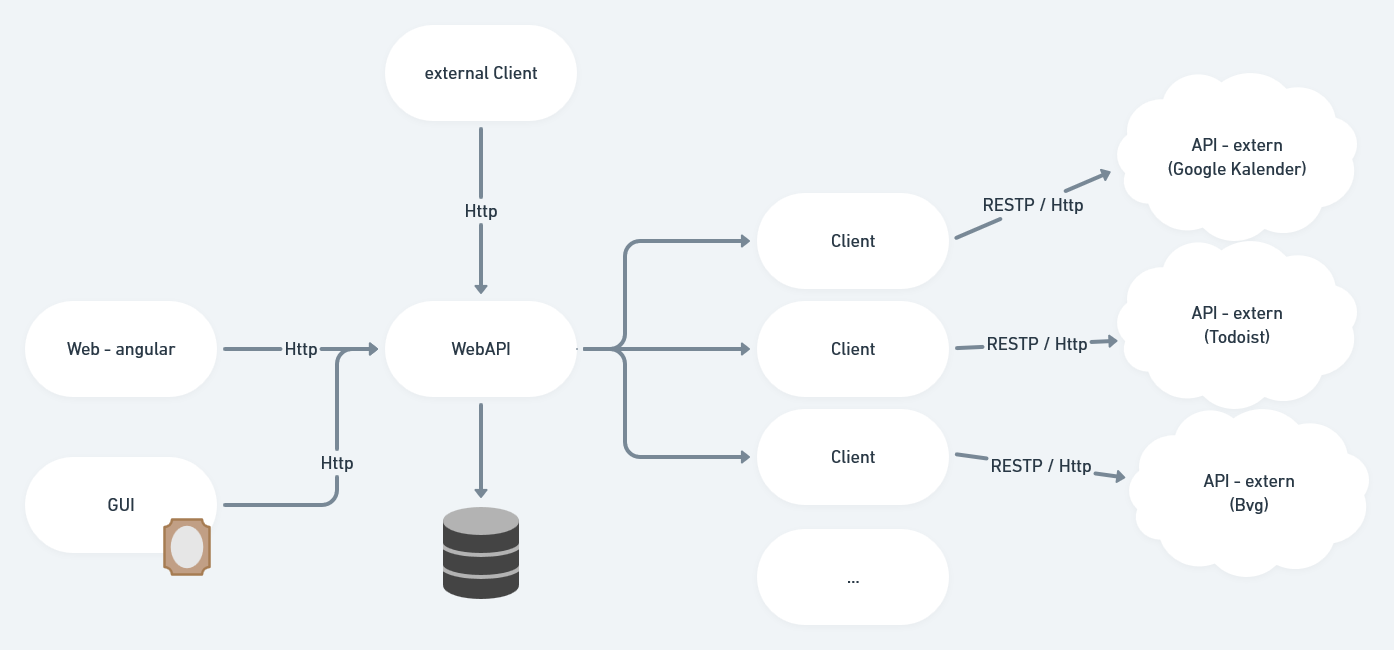
\includegraphics[width=150mm]{pictures/Scalability.png}
\caption{konzeptioneller Aufbau der Software-Komponenten}
\end{figure}\\\
Nach meheren Skizzen und Umgestaltungen kamen wir dann auf diesen Aufbau unserer Software. Auf dem RasperbryPi laufen die folgenden Komponenten: Web - angular, GUI,WebApi, Datenbank und die Clients (mehr zu den einzelnen Komponenten finden sie im Kapitel \ref{Komponenten}). \\\
Die Clients übernehmen die Kommunikation zu den externen Dienst-Anbietern über deren APIs. Die WebAPI organisiert die gesamten anfallenden Daten, wie zum Beispiel: Client-Daten, Benutzerdaten und GUI-Elemente. Auserderm organisiert sie die einzelnen Clients mit deren dazugehörige API und stellt ein eigene API bereit über die Daten abgefragt werden können. Diese API nutzt wiederrum das Frontend, also die GUI Komponente und die Web Komponente. Die GUI ist für die Ansicht auf dem Display hinter dem Glass zuständig. Sie fragt die Daten vom aktuellen Benutzer über die WebAPI ab und formt diese Daten zu einer Ansicht. Die Web Komponente stellt einen Web-Service zur Verfügung, sodass der Benutzer über ein Web-Interface über ein mobiles Endgerät Einstellungen vornehmen kann. Dort kann er Einstllungen bezüglich verschiedener Benutzerkonten und deren Dienste machen. Diese API kann natürlich auch von externen Clients benutzt werden, um zum Beispiel mit eigene SmartHome Produkte mit dem SmartMirror zu interagieren oder den SmartMirror zu steuern.\\\

Um den SmartMirror (RaspberryPi) ins eigene WLAN zu bringen haben wir uns folgende Methodik überlegt. Der RaspberryPi stellt über den integrierten Wifi-chip ein eigenes WLAN zur Verfügung. In dieses muss sich der Benutzer zur Konfiguration einwählen. über ein kleines Web-Interface soll er dann sein WLAN auswählen und das Passwort eingeben oder den SmartMirror über den eigenen WLAN Router freischalten.


\subsubsection{Benutzerfreundlichkeit}\label{Benutzerfreundlichkeit}
Die eigentliche Idee dabei ist den Spiegel nicht einfach nur spiegeln zu lassen oder die Uhrzeit anzeigen zu lassen, sondern ihn "smart" zu machen, sodass man ihn praktischen und effizient Nutzen kann. Zudem war uns auch wichtig, dass es \textbf{Benutzerfreundlich} ist, da nicht jeder das Know-How hat sich einen Spiegel für seine Eigenen Bedrüfnisse zusammen zu bauen bzw. zu programmieren. Er sollte einfach und verständlich für jeden sein. Deshalb haben wir auch die in das Konzept die Web Komponente eingefügt und die GUI leicht erweiterbar gestaltet.

\subsubsection{Skalierbarkeit}\label{Skalierbarkeit}
Der SmartMirror ist nicht nur Benutzerfreundlich, sondern ist auch in vielen Richtungen skalierbar.
Wie schon erwähnt, wollten wir die bereits bestehenden Dienste Nutzen. Zum Beispiel hat man seine Kalendereinträge bereits im Google-Kalender eingetragen und hat keine Lust als Kunde alle Daten auf den Kalender des SmartMirrors zu übertragen. Es wäre für den Benutzer leichter auf diese Daten zuzugreifen. \\\
Viele Anbieter von Diensten stellen über das Http-Protokoll API Funktionen für Ihren Dienst bereit. Diese API's nutzt der SmartMirror, um dann die Daten vom dem jeweiligem Dienst abfragen zu können. Dieses Abfragen geschieht in der Client Komponente, auf welche wir näher im Kapitel \ref{Clients} Clients eingehen werden. Dadurch ist das System erweiterbar und hilft sogar beim Vernetzen von anderen Diensten.\\\
Neben der Erweiterbarkeit haben wir auch daran gedacht, eine eigene Schnittstelle zu definieren, sodass andere SmartHome-Produkte sich an den SmartMirror vernetzen können. Diese können dann wie die GUI und Web Komponente, Daten vom SmartMirror abfragen oder senden, sodass es zum Beispiel auch denkbar wäre mehrere SmartHome-Produkte so miteinander zu vernetzen, dass der SmartMirror die Basis bildet. Andere SmartHome Produkte könnten in Kooperation\\\




